\documentclass{article}

% Language setting
% Replace `english' with e.g. `spanish' to change the document language
\usepackage[french]{babel}
\usepackage[T1]{fontenc}

% Set page size and margins
% Replace `letterpaper' with `a4paper' for UK/EU standard size
\usepackage[a4paper,top=2cm,bottom=2cm,left=3cm,right=3cm,marginparwidth=1.75cm]{geometry}

% Useful packages
\usepackage{amsmath}
\usepackage{graphicx}
\usepackage[colorlinks=true, allcolors=blue]{hyperref}

% Other packages
\usepackage[indent]{parskip}

\title{Mini-projet 1}
\author{Kataevskii Mikhail, Ahrend Laurentin-Wilhelm, Garcia Harlouchet Ivan, \\ Galliot Noémie, Duhautois Lucas}

\begin{document}
\maketitle

\section{Présentation}

Le verre est un matériau d'avenir, recyclable à l'infini, mais sa production reste encore très polluante, notamment à cause de l'eau utilisée pour refroidir les systèmes et l'énergie dépensée pour chauffer les fours qui servent à la fusion du verre. De plus, les minéraux présent dans la composition initiale du verre relâchent du $CO_2$ lors de leur fusion.

De nombreuses pistes pour pallier à ce problème sont envisagées par les fabriquants, comme augmenter la proportion de calcin (verre recyclé) dans les préparations initiales, ou encore passer de fours à gaz à des fours électriques; mais les progrès faits sont encore loin d'être satisfaisant.

Le but de ce mini-projet est donc d'étudier une manière de réduire les émissions lors de la fabrication du verre. Pour cela, nous nous sommes concentrés sur la température de fusion de ce dernier. En effet, abaisser la température de fusion du verre signifie abaisser l'énergie nécessaire à sa fabrication. Cela permettrait aux entreprises de réaliser des économies d'énergies tout en diminuant leurs émissions. Cependant, le verre ainsi obtenu doit répondre au cahier des charges des entreprises et ne pas perdre en propriétés telles que sa dureté, sa flexibilité ou encore son élasticité.

Afin de répondre à cette problématique, nous disposons d'une base de données \textit{Interglad} regroupant les compositions et les propriétés de plusieurs centaines de milliers de verres.

Notre objectif est de développer un algorithme génétique exploitant cette base de données afin de trouver une composition de verre qui permet de minimiser la température de fusion tout en conservant les propriétés exigées. En effet, si il existe de nombreux algorithme visant à prédire les propriétés du verre à partir de sa composition, il n'en existe pas qui permette de prédire une composition optimale à partir de propriétés spécifiques.

La composition ainsi obtenue sera utilisée pour créer notre propre verre, sur lequel nous pourrons expérimenter afin de tester ses capacités.

\section{Utilisation d'un algorithme de Deep Learning}
\subsection{Les propriétés recherchées}

Nous disposons de plusieurs modèles entraînés sur la base de données \textit{Interglad} qui permettent de prédire les propriétés du verre à partir de sa composition. Nous cherchons à déterminer un verre dont les fractions molaires vérifient :

\begin{itemize}
    \item $0,3 < x_{Si} < 0,75$
    \item $0,1 < x_{Na_2O} < 0,29$
    \item $x_{CaO} < 0,35$
    \item $x_{Al_2O_3} < 0,23$
\end{itemize} 

Nous cherchons à obtenir un verre qui possède les propriétés suivantes :

\begin{itemize}
    \item $1200 ^{\circ} C < T_m < 1300 ^{\circ} C$
    \item $2300 \text{ kg} \cdot \text{m}^{-3} < \rho < 2800 \text{ kg} \cdot \text{m}^{-3}$
    \item $500 ^{\circ} C < T_g < 600 ^{\circ} C$
    \item $70 < E < 90$
\end{itemize}

Pour fabriquer le verre nous avons accès aux composants suivantes : $SiO_2$, $Al_2O_3$, $MgO$, $CaO$, $Na_2O$, $K_2O$, $ZnO$, $TiO_2$

\subsection{Optimisation à partir de composants de base}

Nous avons d'abord cherché une composition optimale en se limitant aux 3 composants de base que l'on retrouve dans la plupart de verres : $SiO_2$, $NaO_2$ et $CaO$. Pour cela nous avons modifié la fonction de tirage au sort pour se limiter aux mélanges de ces 3 éléments. Nous avons ensuite trié la liste de compositions obtenues afin de trouver celle qui correspond le mieux à nos exigences.

La composition obtenue a été utilisée pour la première fusion du verre.

\subsection{Elaboration d'un algorithme génétique}
%TODO

\section{Fonte d'un premier verre}
\subsection{Composition}

En analysant les bases de données fournies par nos encadrants et celles sur Interglad, nous avons déterminé une première composition de verre, à l'aide uniquement de $SiO_2$, de $CaO$ et de $Na_2O$. Cette composition molaire est la suivante:

\begin{itemize}
    \item 65,4 \% de $SiO_2$
    \item 11,3 \% de $CaO$
    \item 23,3 \% de $Na_2O$
\end{itemize}

Les propriétés de ce verre prédites par la base de données sont les suivantes:
\begin{itemize}
    \item Température de fusion: Tm = 1258°C
    \item Température de transition vitreuse: Tg = 502 °C 
    \item Module de Young: E = 73,6
    \item Masse volumique: 2,57 $g/cm^{3}$ \\
\end{itemize}

Cette composition est très proche de celle utilisée par les égyptiens il y a plus de 2500 ans, d’après les écrits de la bibliothèque du roi Assurbanipal (70 \% de $SiO_2$, 10 \% de $CaO$, 20\% de $Na_2O$), car le verre est connu depuis très longtemps et sa composition a peu varié. 

En effet, un verre est composé des trois éléments principaux:
\begin{itemize}
    \item un formateur : Le formateur de verre forme la structure du verre. Il s'agit ici de $SiO_2$.
    \item Un fondant : Les fondants permettent la réduction de la température de fusion du verre en rompant certaines liaisons entre les molécules du formateur. Il s'agit ici de $Na_2O$
    \item Un ou plusieurs modificateur(s) de réseaux : Les modificateurs de réseaux permettent d'améliorer les propriétés du verre telles que la durabilité chimique ou mécanique. Il s'agit ici de $CaO$.
\end{itemize}

Les trois composants utilisés pour cette première compositions sont les composants les plus classiques, du fait de leurs rôles respectifs dans la formation du verre. Il n'est donc pas étonnant de retrouver une composition similaire à celle utilisée il y a déjà plusieurs milliers d'années. 

Par la suite, nous tenterons d'élaborer un verre plus complexe, notamment à l'aide d'ajouts d'oxides de minéraux.

\subsection{Fusion du mélange}

Les proportions citées ci-dessus ont ensuite été converties en proportions massiques, afin de réaliser le mélange à l'aide d'une balance de précision. Après homogénéisation, le mélange est introduit dans un creuset, lui-même inséré dans un support, avant d'être mis dans un four électrique, de modèle RHF 14/15 (voir en annexe ses capacités). Le support du creuset a été taillé afin d'avoir la même taille que ce dernier et ainsi permettre une meilleure prise pour la pince à la sortie du four.

Le protocole de fusion du verre est donné en annexe. Pour des raisons techniques de taille du creuset, la fonte est réalisée en deux parties. Une première partie du mélange est fondue puis une deuxième partie du mélange est réintroduite dans le liquide, et la fusion se poursuit.

Le liquide obtenu est ensuite coulé dans un moule en acier rectangulaire. Le verre ainsi obtenu est laissé à refroidir à l'air libre.

Toutes les manipulations en contact direct avec le four à de très hautes températures ont été réalisées par Franck Pigeonneau et Cristophe Prady, à l'aide d'équipements de protections contre ces températures.

\subsection{Recuisson du verre}

Le verre obtenu a été refroidi à température ambiante. Cependant, ce refroidissement a donc été inhomogène, plus rapide à l'extérieur qu'à l'intérieur. Cela a induit des contraintes, fragilisant le verre.

Pour pallier à ce problème, le verre est donc recuit. Il est enfourné dans un four dont la température est celle de sa transition vitreuse, soit environ 500°C. Le four est éteint et laissé à refroidir toute la nuit avec le verre à l'intérieur.
Cette étape permet la suppression des contraintes.

Nous avons ainsi obtenu notre premier verre.

\begin{figure}[h]
    \centering
    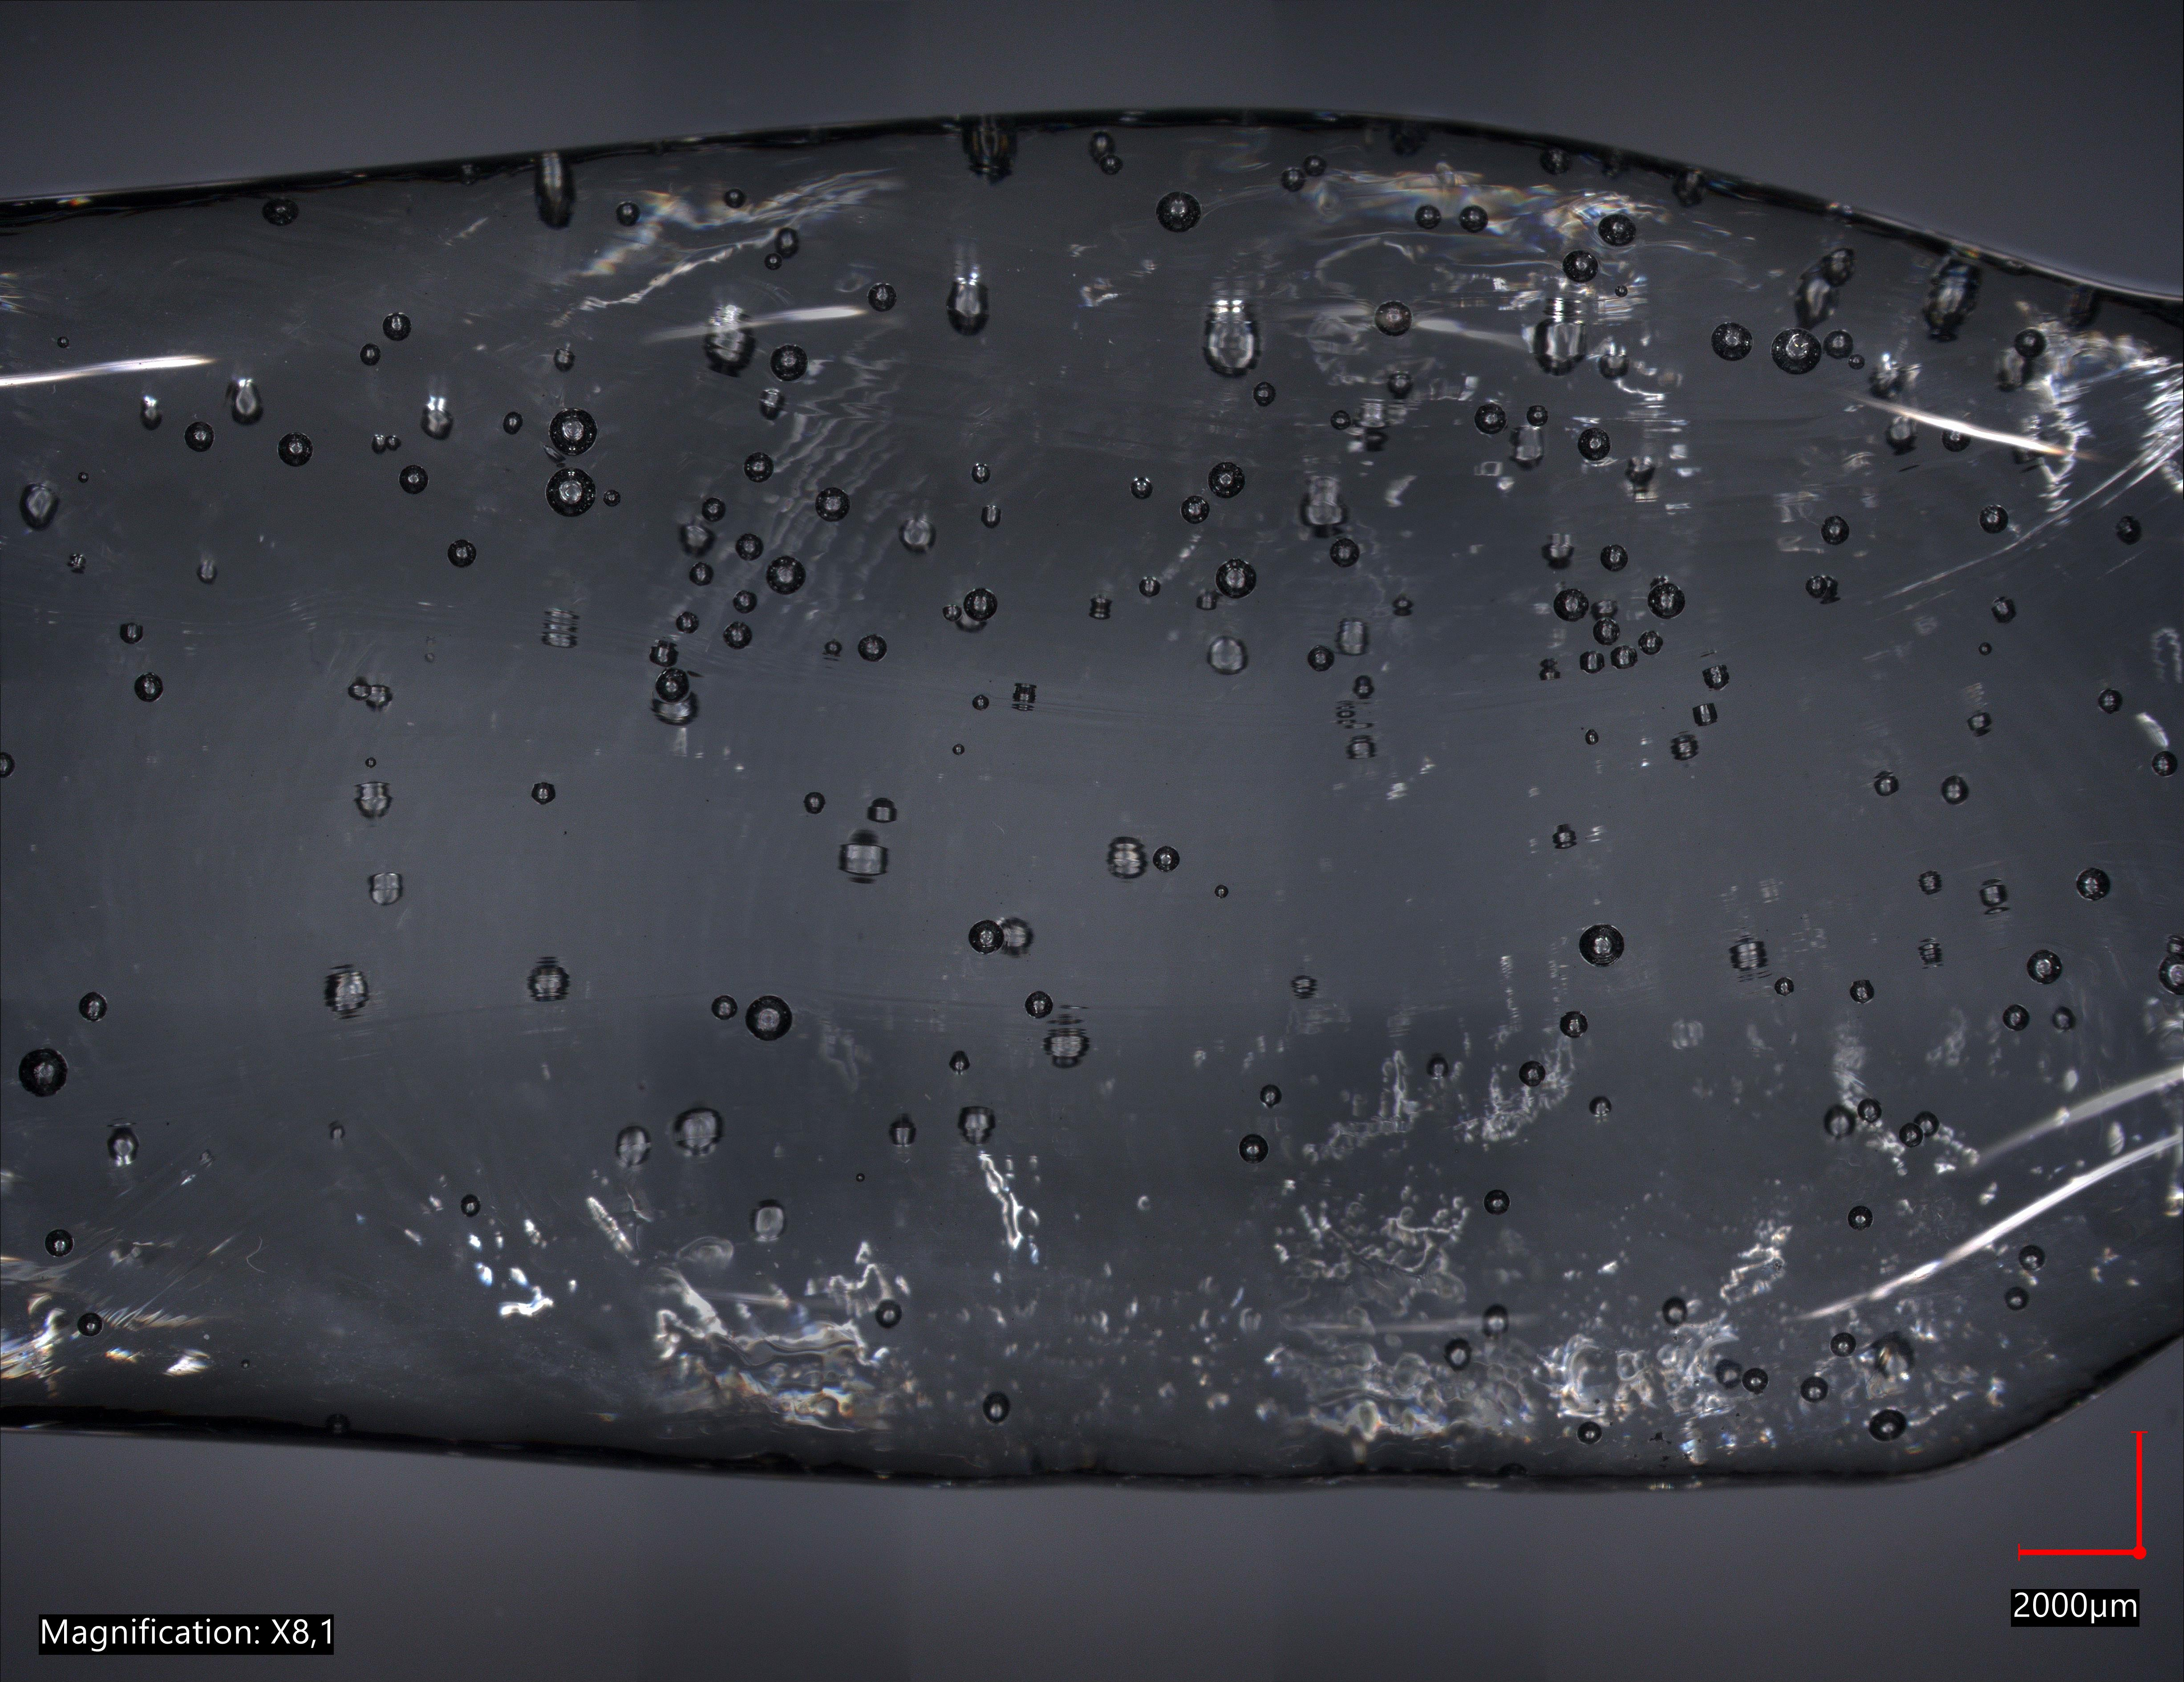
\includegraphics[width=0.5\textwidth]{photos/mosaic.jpg}
    \caption{photographie au microscope optique du verre issu de la première fusion}
\end{figure}

\subsection{Analyse des propriétés du verre}

\subsubsection{Observation des contraintes}
Le verre obtenu est ensuite analysé. Il est tout d'abord exposé à de la lumière polarisante afin de vérifier si les contraintes ont bien disparue.

\begin{figure}[h]
    \centering
    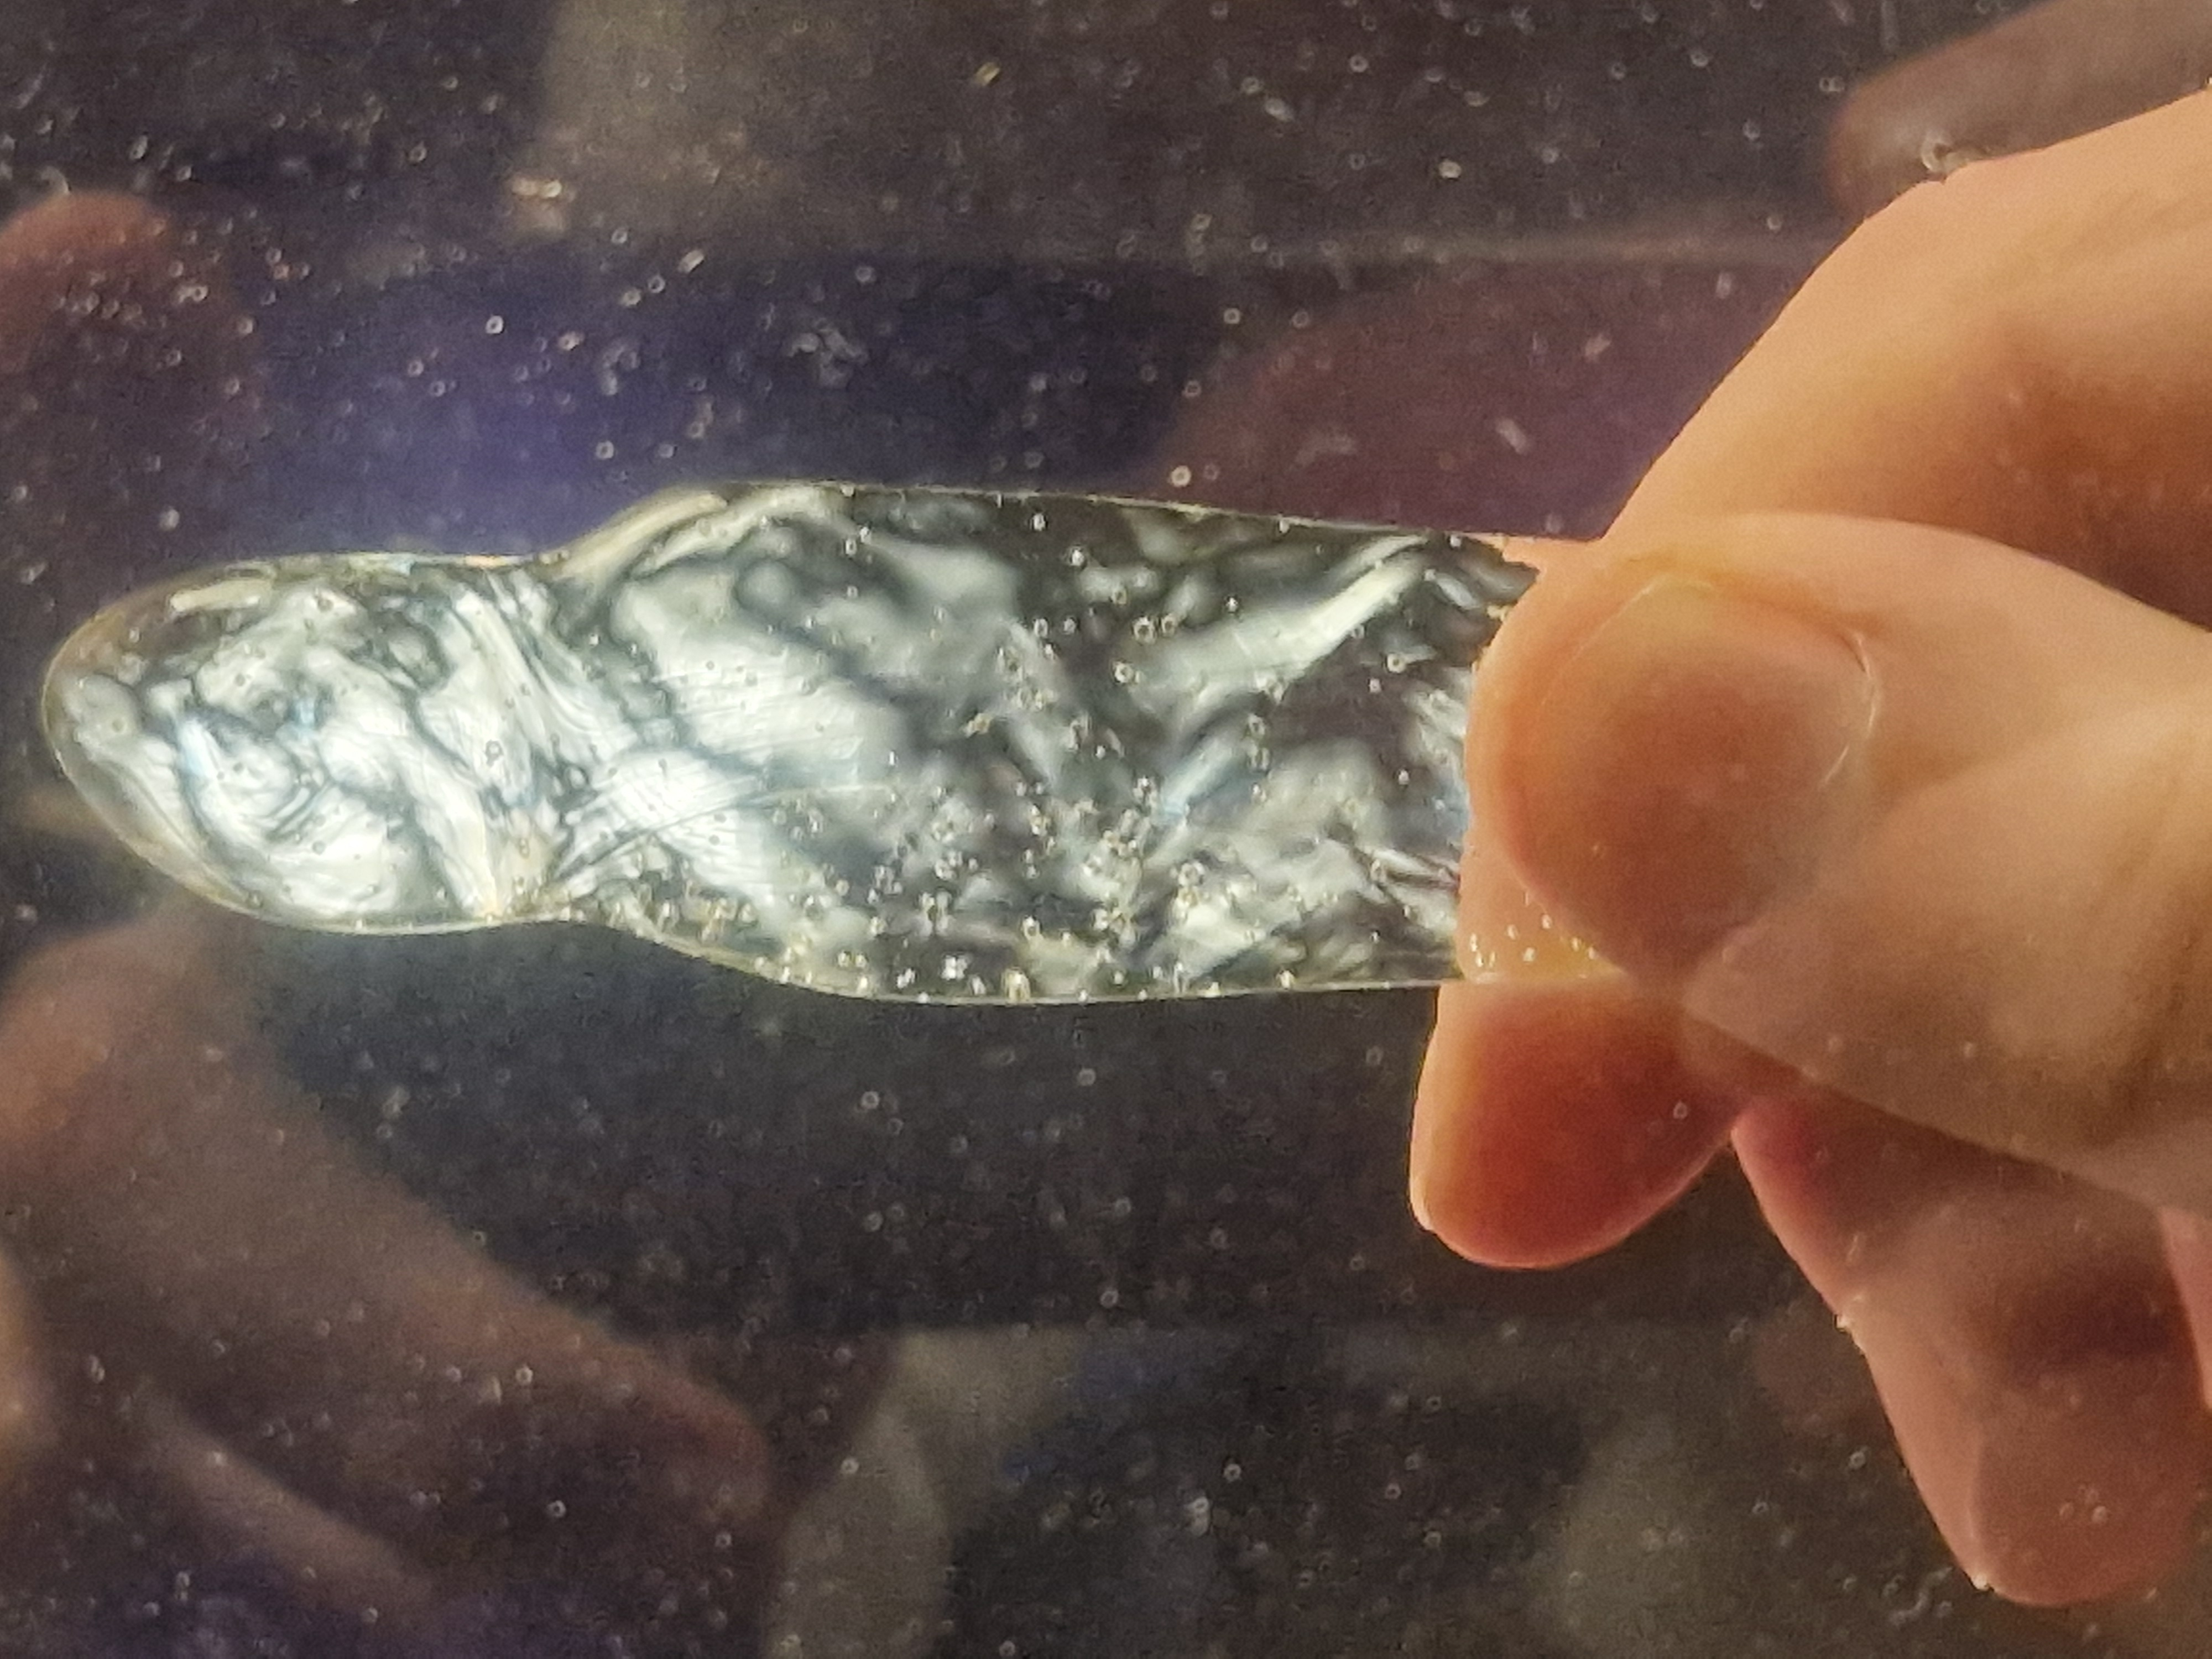
\includegraphics[width=0.5\textwidth]{photos/contraintes.jpg}
    \caption{observation des contraintes dans le verre à la lumière polarisée}
\end{figure}


[On n'observe pas de colorisation ce qui indique bien l'absence de contrainte]

\subsubsection{Observation au microscope optique}

Il est ensuite observé au microscope optique, où l'on peut voir la présence de rares infondus. Ce passage au microscope optique nous a permis également d'observer les bulles présentes dans le verre et de les compter.

\begin{figure}[h!]
    \centering
    \begin{minipage}{0.45\textwidth}
        \centering
        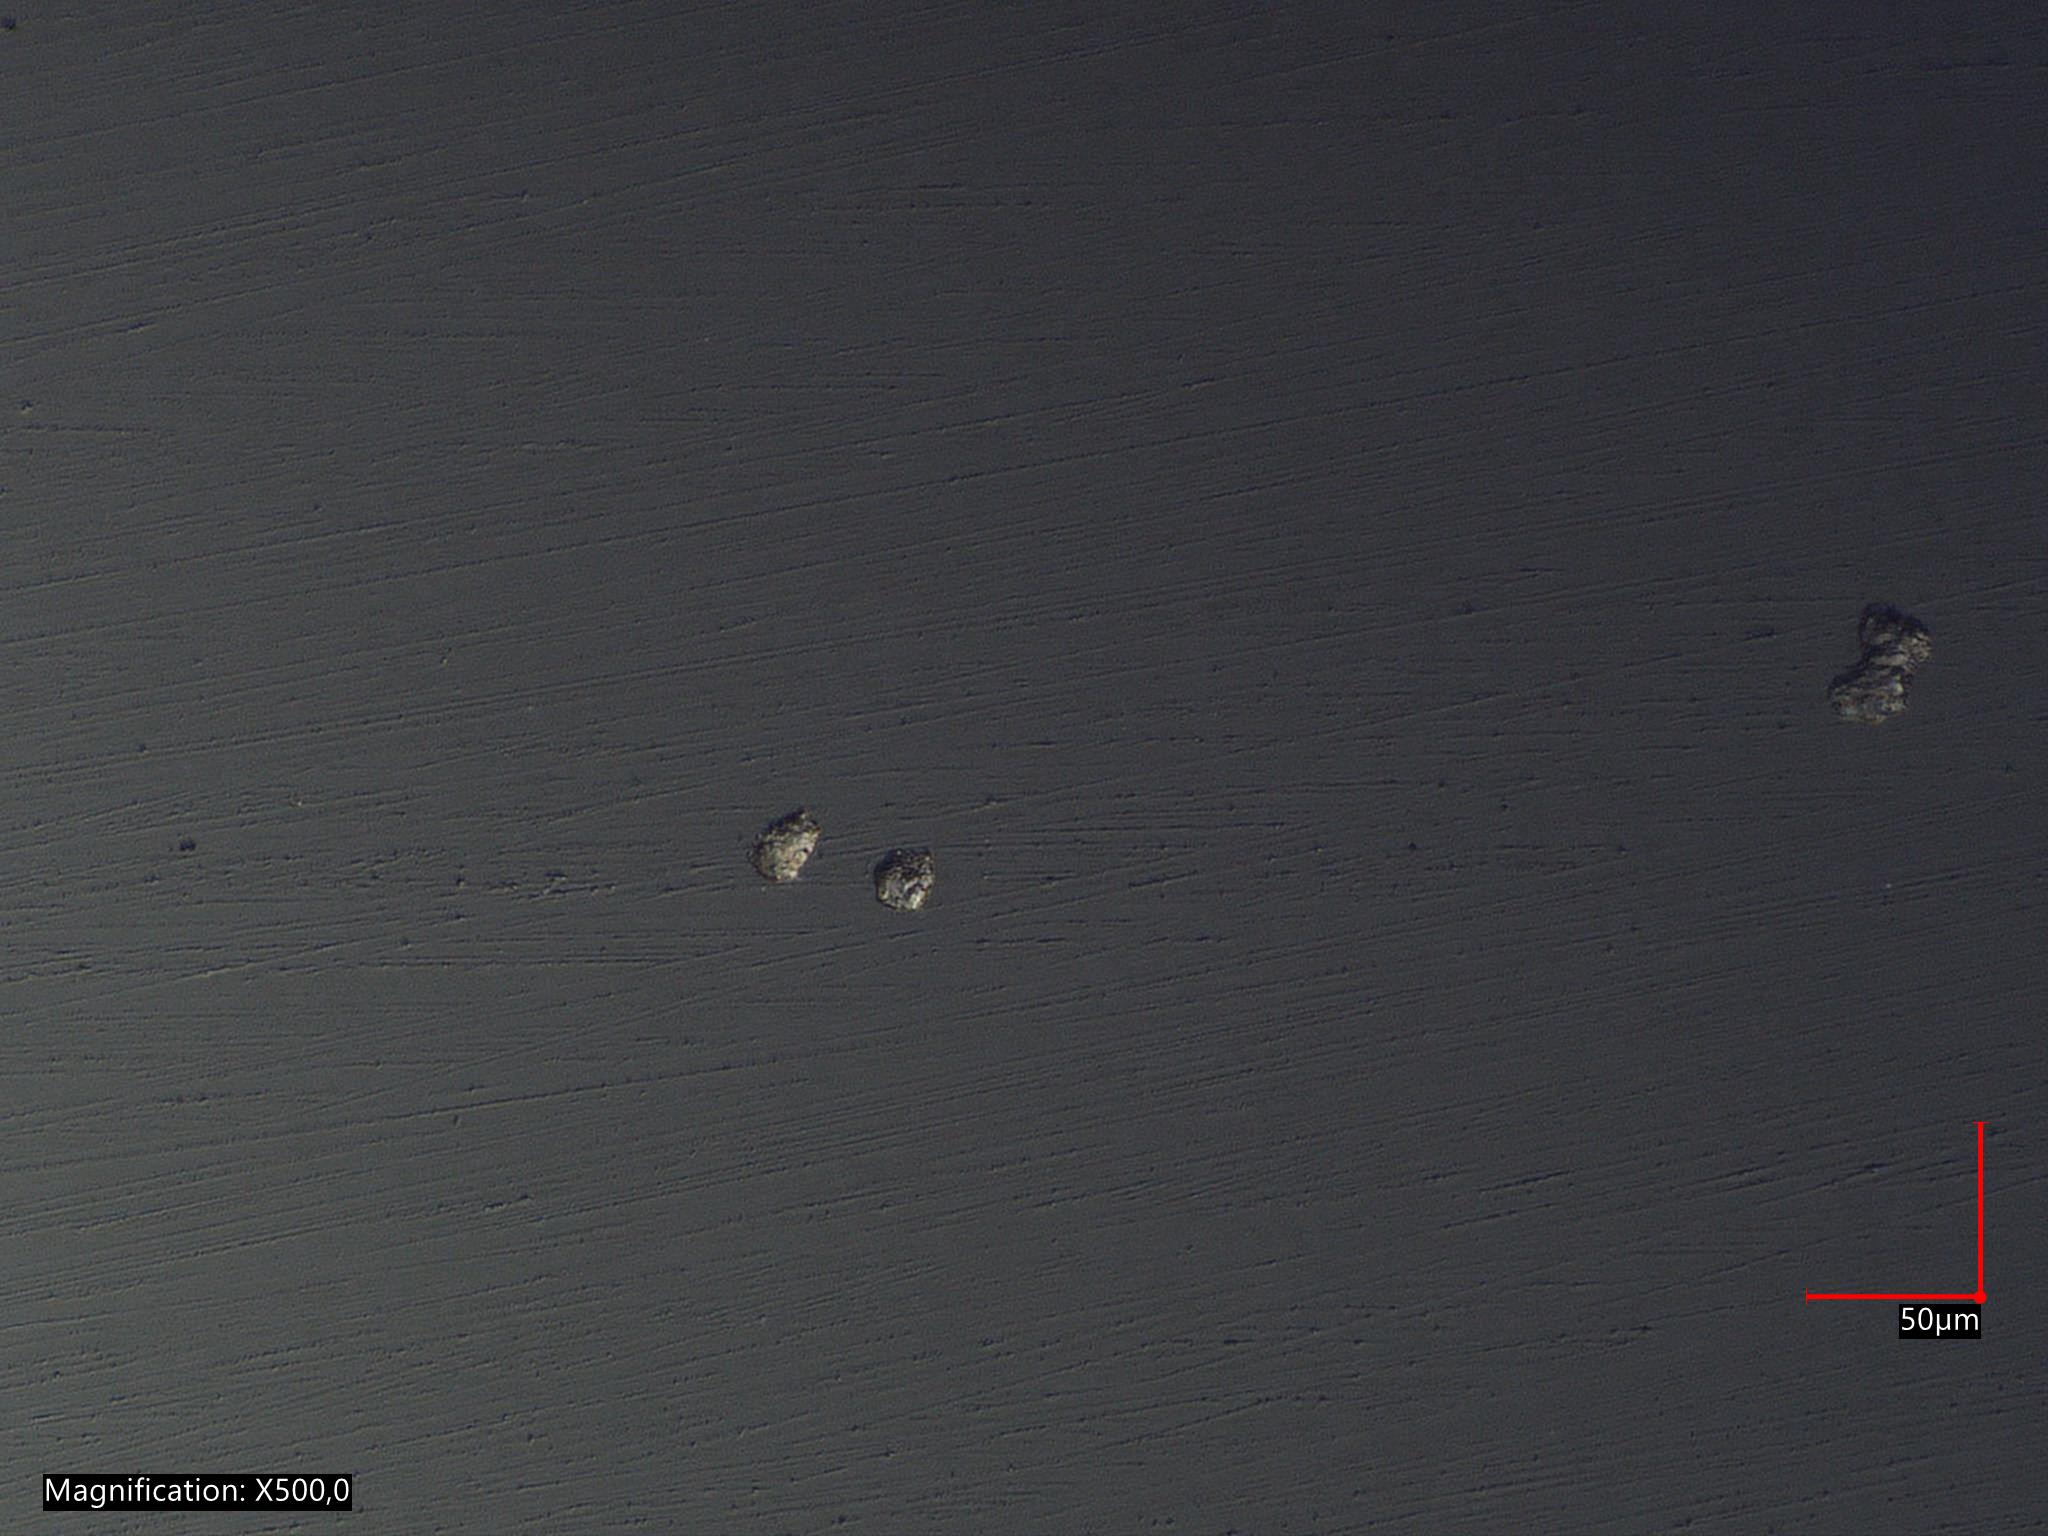
\includegraphics[width=\textwidth]{photos/impuetée2.jpg}
        \caption{infondus observés au microscope optique}
    \end{minipage}
    \hspace{0.5cm}
    \begin{minipage}{0.45\textwidth}
        \centering
        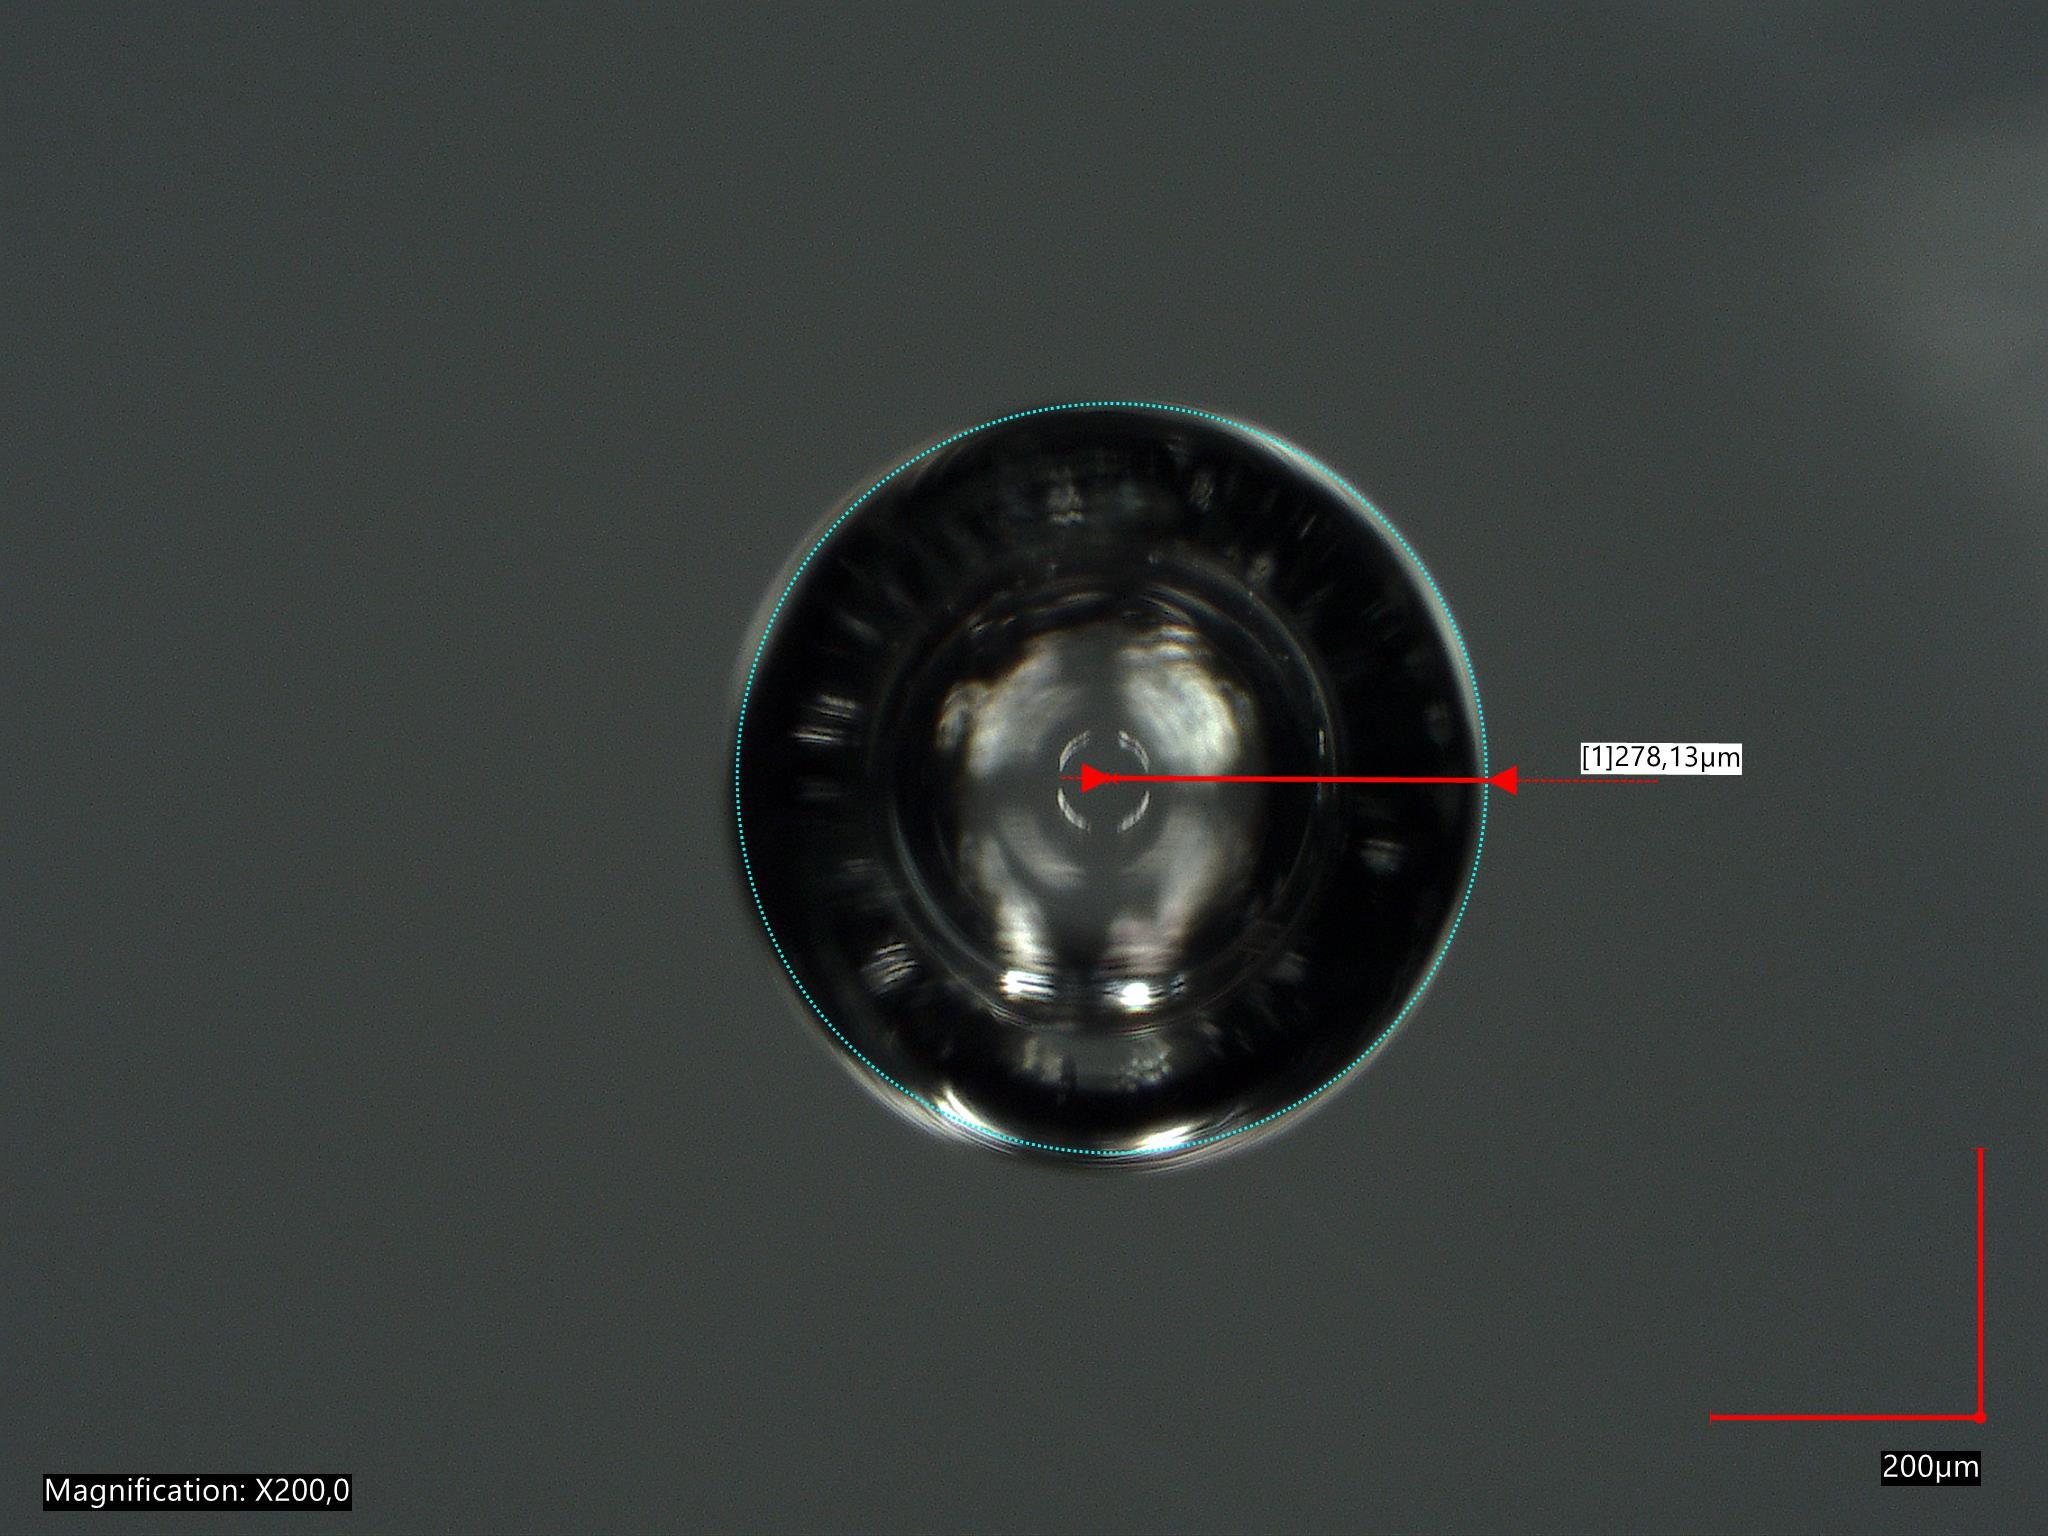
\includegraphics[width=\textwidth]{photos/rayon 1.jpg}
        \caption{Bulle d'air observée au microscope optique}
    \end{minipage}
\end{figure}

Les bulles d'airs sont dues à la viscosité importante du verre, d'environ 1000 fois celle de l'eau lorsque le verre est en fusion. En effet, les bulles d'air sont donc piégées et s'échappent lentement. Pour un verre sans bulles, il aurait fallu maintenir la fusion pendant plus longtemps. Dans les fours industriels, le verre en fusion reste en moyenne plusieurs jours dans les fours.

\subsubsection{Mesure de dureté et de densité}

Le verre a ensuite été découpé afin de pouvoir mesurer sa dureté de Vicker et sa densité. 


\begin{figure}[h]
    \centering
    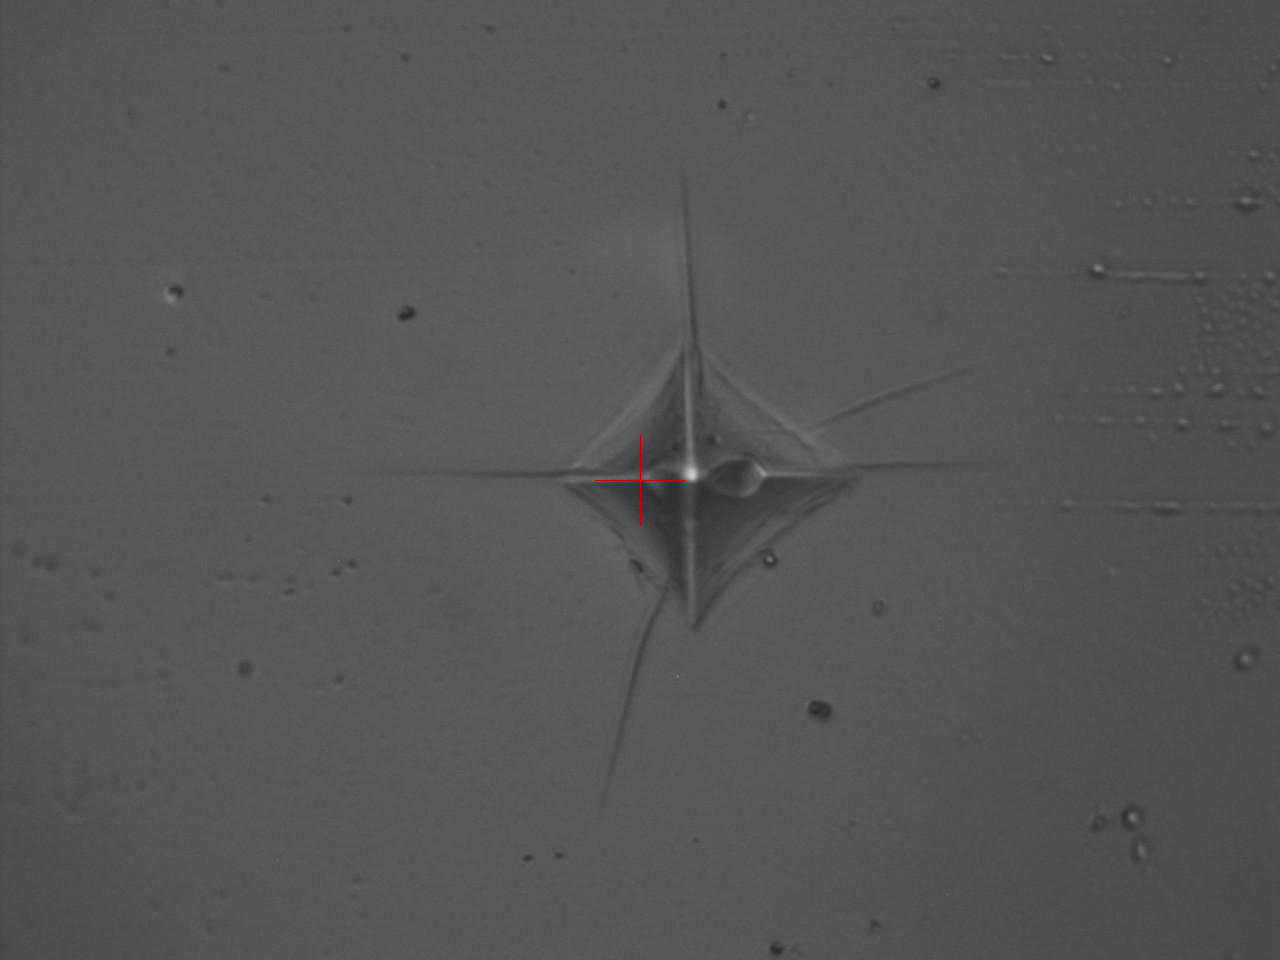
\includegraphics[width=0.5\textwidth]{photos/dureté.jpg}
    \caption{Mesure de la dureté de Vicker}
\end{figure}

[Cette mesure est effetuée en enfoncant un poinçon en diamant dans le verre et en mesurant la taille de la marque, ici pour 200g de charge on a une durabilité de vickers de 536 HV c'est une valeur cohérente pour du verre mais pas particulièrement impressionante]


La densité du verre a été mesurée à l'aide d'un densimètre, utilisant une balance de précison pour mesurer la masse et des particules fines pour mesurer le volume. 

\section{Fusion d'un verre plus complexe}

\subsection{Composition}

Nous avons réalisé un algorythme génétique utilisant le réseau de neurones fournis par notre encadrant afin de trouver une nouvelle composition. 

\begin{itemize}
    \item 53,4 \% de $SiO_2$
    \item 3,51 \% de $CaO$
    \item 18,7 \% de $Na_2O$
    \item 2,13 \% de $Al_2O_3$
    \item 2,65 \% de $MgO$
    \item 9,44 \% de $ZnO$
\end{itemize}

Les propriétés de ce verre prédites par l'algorithme génétique sont les suivantes:
\begin{itemize}
    \item Température de fusion: Tm = 1154°C
    \item Température de transition vitreuse: Tg = 563 °C 
    \item Module de Young: 81,2
    \item Masse volumique: 2,81 $g/cm^{3}$
\end{itemize}

\subsection{Fusion du verre}

Le verre est mis dans un four déjà à la température de 1200°C.

\section{Annexe mini-projet 1}
\subsection{Protocole de fusion du verre}

Lors de la fusion du verre, nous avons suivis le protocole suivant :

\begin{enumerate}
    \item Préparation de la composition
    \item Enfournement d'une première partie du mélange vitrifiable
    \item Montée en température du four à 900°C
    \item Palier de 30 minutes
    \item Montée en température du four à Tm en 60 minutes
    \item Maintien de la température pendant 1h
    \item Enfournement du reste de la composition
    \item Remise en température à Tm pour 1h
    \item Coulée du verre dans un moule
\end{enumerate}

\subsection{Capacités du four électrique utilisé pour la fusion}

Les informations ci-dessous ont été fournies par le fabriquant (Carbolite) sur son site internet.

\begin{tabular}{|c|c|}
\hline
Température maximale (°C) & 1400  \\
\hline
Volume (L) & 15 \\
\hline
Temps de chauffe (min) & 35 \\
\hline
dimension interne HxLxP (mm) & 220x220x310 \\
\hline
Dimension externe HxLxP (mm) & 810x690x780 \\
\hline
Puissance max (W) & 10 000 \\
\hline
Puissance de maintien à température (W) & 2900 \\
\hline
Poids (kg) & 125 \\
\hline
\end{tabular} 


\end{document}
